\subsection{\label{sec:A22}Hochohmiges Silizium}
Nun betrachten wir den THz-Puls nach Propagation durch hochohmiges Silizium (HR-Si).
Der dünne Wafer wird in einen Probenhalter geklemmt und am Probentisch befestigt. Zur Aufnahme 
werden folgende Messparameter gewählt
\begin{equation}
    \Delta s = 0,001\,\si{mm}, \hspace{1.5cm} N_{\text{s}} = 2500, \hspace{1.5cm} N_{\text{sample}} = 100, \hspace{1.5cm} s_{0} = 152,7\,\si{mm}.
\end{equation}
Zudem wir die Dicke des Wafers mithilfe eines Messschiebers ($d_{\text{mess}}$) bestimmt. 
Der auftretende Etalon-Effekt (siehe Abb.~\ref{fig:HR}), der durch Reflexion des THz-Pulses 
an der Grenzschicht des HR-Si 
entsteht, kann zudem genutzt werden, um die Dicke der Probenschicht zu bestimmen. 
Hierzu betrachten wir die Maxima des primären und des sekundären Pulses und errechnen aus 
der zeitlichen Verzögerung die gewünschte Größe
\begin{align}
    v &= \frac{s}{t} \\
    \Rightarrow \frac{c}{n_{\text{Si}}} &= \frac{2d_{\text{etalon}}}{t_{2} - t_{1}} \\
    \Leftrightarrow d_{\text{etalon}} &= \frac{c}{2n_{\text{Si}}}\left(t_{2} - t_{1}\right) \\
    s_{d_{\text{etalon}}} &= \sqrt{2\left(\frac{c}{2n_{\text{Si}}}s_{t_{1,2}}\right)^{2}}.
\end{align} 
Mit $n_{\text{Si}} = 3,4175$ \cite{Anleitung}, den Messwerten für die betrachteten Zeitpunkte, 
sowie dem hierzu abgeschätzten Ablesefehler folgt 
\begin{equation}
    t_{1} = (4,887 \pm 0,007)\,\si{ps} \hspace{2.5cm} t_{2} = (11,067 \pm 0,007)\,\si{ps}
\end{equation}
\begin{equation}
    \Rightarrow\fbox{$d_{\text{etalon}} = (271,1 \pm 0,4)\,\si{\mu m}$}.
\end{equation}
Der Vergleich der Verzögerung des THz-Pulses zwischen Referenz und HR-Si, liefert eine 
weitere Methode zur Bestimmung der Dicke. Aus Gl.~\eqref{eq:a22} folgt der relevante Zusammenhang zu
\begin{equation}
    d_{\text{ref}} = \frac{c}{(n_{\text{Si}} - 1)}\left(t_{1} - t_{3}\right),
\end{equation}
wobei $t_{3}$ der zeitlichen Verzögerung entspricht, bei der der Referenzpuls maximal wird. 
Wir erhalten
\begin{equation}
    t_{3} = (2,653 \pm 0,007)\,\si{ps}
\end{equation}
und damit schlussendlich 
\begin{equation}
    \Rightarrow\fbox{$d_{\text{ref}} = (277,0 \pm 1,2)\,\si{\mu m}$}.
\end{equation}
Die Ergebnisse sind abschließen im Vergleich zur Herstellerangabe $d_{\text{prod}}$ aufgelistet
\begin{equation*}
    \fbox{$d_{\text{prod}} = (280 \pm 10)\,\si{\mu m},\hspace{0.4cm}
    d_{\text{mess}} = (270 \pm 5)\,\si{\mu m},\hspace{0.4cm}
    d_{\text{etalon}} = (271,1 \pm 0,4)\,\si{\mu m},\hspace{0.4cm}
    d_{\text{ref}} = (277,0 \pm 1,2)\,\si{\mu m}$}.
\end{equation*} 
Es ist zu sehen, dass alle Ergebnisse in der gleichen Größenordnung liegen und innerhalb des Fehlers
mit der Herstellerangabe überlappen. Die Fehlerangabe der mittels THz-TDS errechneten Ergebnisse 
beinhaltet nur Ablesefehler der Messungen und berücksichtigt keinerlei Fehler im 
Messaufbau. Hiernach kann der Fehler größer geschätzt werden, was in einer noch besseren 
Übereinstimmung aller gemessenen Dicken resultiert. \\ \\
Weiterhin betrachten wir das Amplituden-Transmissionsspektrum $T(\omega)$, welches sich aus 
dem Quotienten der spektralen Amplituden der Probe $\left\vert E_{\text{sample}}(\omega) \right\vert$
und der Referenz $\left\vert E_{\text{ref}}(\omega) \right\vert$ ergibt. 
Hierzu muss zunächst der gemessene THz-Puls Fouriertransformiert werden, was einige technische 
Zwischenschritte benötigt. 
Zuerst wird der relevante Bereich des Pulses herausgeschnitten, was im Falle des HR-Si einem Abschneiden 
des sekundären Pulses entspricht. Dieser würde nach Abschnitt \ref{subsec:FZV7} zu einer Änderung der
untersuchten Transmission führen. Dieser Bereich muss nun, durch Anhängen von Nullen im Signal, 
um das Pulsmaximum symmetrisiert werden. Um das Signal zu verbessern und Artefakte in der Frequenzdomäne 
zu reduzieren wird dieses symmetrisierte Zeitsignal mit einer Fensterfunktion multipliziert, um sicherzustellen, 
dass das transformierte Signal periodisch ist. Um schließlich die Frequenzauflösung im reziproken Raum 
zu verbessern werden bei der Fourier-Transformation weitere Nullen 
ans Signal angehängt (siehe Abschnitt \ref{subsec:FZV5}). 
Das errechnete Ergebnis ist stark vom vorangegangenen Verarbeitungsprozess abhängig, was eine 
Vergleichbarkeit erschwert. Für unsere Auswertung wird die Hamming-Fensterfunktion gewählt, für 
welche gilt \cite{Wiki}
\begin{equation}
    \mathcal{H}(n) = 0,54-0,46\cos(\frac{2\pi n}{N-1}),
\end{equation}
wobei $N$ die Signallänge angibt und $n$ dem Index entspricht, der über das Signal läuft. \\
In Abb.~\ref{fig:HR} ist der gemessene THz-Puls nach Durchgang durch das HR-Si, der Referenzpuls 
und die Transmission dargestellt.
\begin{figure}[h!]
    \centering
    \subfloat[\centering gemessene THz-Pulse]{{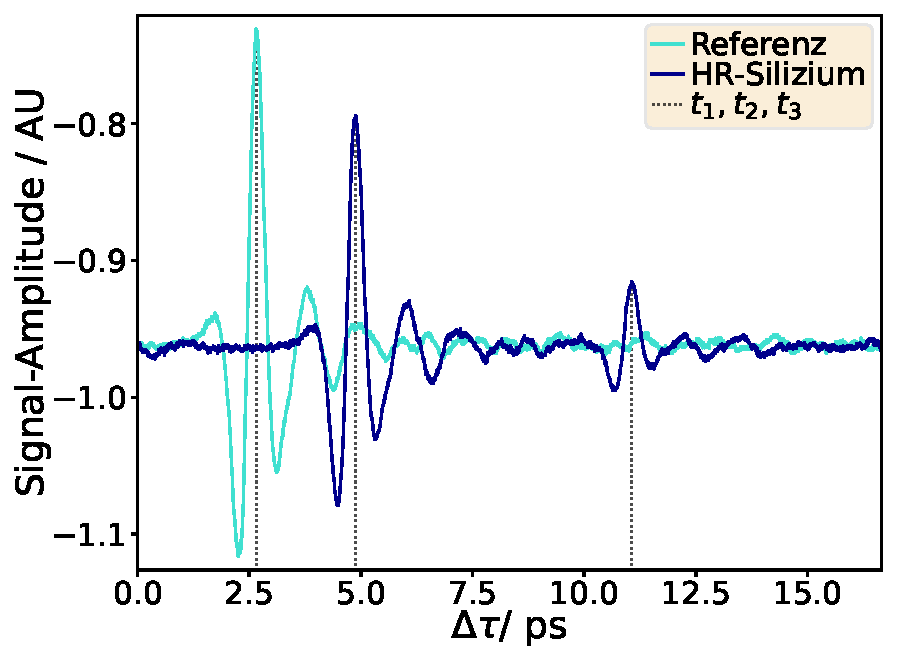
\includegraphics[width=0.47\textwidth]{HRPuls.pdf} }}
    \qquad
    \subfloat[\centering Amplituden-Transmissionsspektrum]{{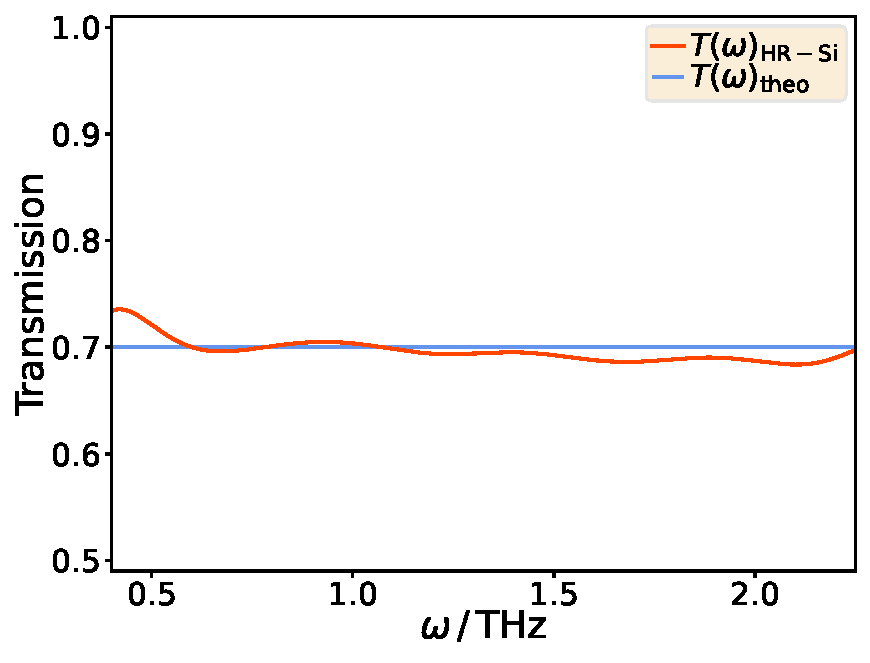
\includegraphics[width=0.47\textwidth]{HRTrans.pdf} }}
    \caption{\label{fig:HR}a) Gemessenes THz-Signal des Referenzpulses (hellblau) verglichen 
    mit dem durch den Si-Wafer propagierten Puls (dunkelblau). Zusätzlich sind die zur Dicken-Berechnung verwendeten
    Zeitpunkte $\Delta \tau = t_{1,2,3}$ eingezeichnet. Der Etalon-Effekt ist an dem zweiten 
    schwächeren Signalpuls erkennbar. \\
    b) Das Amplituden-Transmissionsspektrum $T(\omega)$ für HR-Si verglichen mit der theoretischen Erwartung 
    aus der vorbereitenden Frage \ref{subsec:FZV7}.}
\end{figure}\FloatBarrier
Für die Berechnung der spektralen Amplituden wurde der relevante Bereich jedes Pulses verwendet. 
Die ermittelte Transmission liegt nahe an der theoretischen Erwartung, zeigt jedoch eine leichte 
Frequenzabhängigkeit. Da bei der Berechnung der Transmission verschiedene Ausschnitte der Pulse 
und unterschiedliche Fensterfunktionen miteinander verglichen wurden und dabei deutliche 
Unterschiede im Ergebnis festgestellt werden konnten, gestaltet sich eine Interpretation der 
Ergebnisse als herausfordernd. Die beobachteten Oszillationen sind vermutlich auf Berechnungs- 
und Messartefakte zurückzuführen, die nicht aus einer Änderung des Brechungsindex oder anderen 
Eigenschaften der Probe resultieren. \\
Insgesamt gewinnen wir Einblicke in die Funktionsweise der THz-TDS und erkennen mögliche 
Herausforderungen bei der Berechnung und Messung. Trotz des gewissen Interpretationsspielraums 
entsprechen die Ergebnisse den Erwartungen und sind daher als zufriedenstellend zu betrachten. \\